\documentclass[11pt,letterpaper]{article}

\usepackage[margin=1in, paperwidth=8.5in, paperheight=11in]{geometry}
\usepackage{authblk}
\usepackage[hidelinks]{hyperref}
\usepackage{setspace}
\usepackage[utf8]{inputenc}
\usepackage{graphicx,float}
\usepackage{amsmath}
\usepackage{siunitx}
\usepackage{indentfirst}
\usepackage[labelfont=bf]{caption}
\usepackage{subcaption}
\usepackage{csquotes}

% Macros
\newcommand{\myTitle}{Application of a U-Net Convolutional Neural Network to Ultrasonic Wavefield Measurements for Defect Characterization}

% Title page
\title{\Large{\textbf{\myTitle}}}
\author[1]{\large{Joshua D. Eckels}}
\author[1]{\large{Isabel F. Fernandez}}
\author[1]{\large{Kelly Ho}} 
\author[2]{\authorcr\large{Nikolaos Dervilis}}
\author[1]{\large{Erica M. Jacobson}}
\author[1]{\large{Adam J. Wachtor}}
\affil[1]{NSEC-EI, Los Alamos National Laboratory, \authorcr Los Alamos, NM 87545 \bigskip}
\affil[2]{Department of Mechanical Engineering, The University of Sheffield, \authorcr Sheffield, UK S10 2TN}
% \affil[1]{Rose-Hulman Institute of Technology, Terre Haute, IN, United States}
% \affil[2]{New Mexico State University, Las Cruces, NM, United States}
% \affil[3]{University of Washington, Seattle, WA, United States}
% \affil[4]{Los Alamos National Laboratory, Los Alamos, NM, United States}
% \affil[5]{The University of Sheffield, Sheffield, England}
\setcounter{Maxaffil}{0}
% \renewcommand\Affilfont{\itshape\small}
\date{\today}

\begin{document}
	\maketitle
%    \thispagestyle{empty}
%    \pagestyle{empty}
    \singlespacing
    \setlength{\parindent}{0in}
    
	\section{Project information}
	The goal of this project is to utilize a U-net style convolutional neural network (CNN) to identify and characterize defects in a plate-like structure. Acoustic wavenumber spectroscopy (AWS) is the current system that takes a 2D, steady-state, out-of-plane surface velocity response of a plate-like structure to a single-tone ultrasonic excitation, (via attached transducer), and identifies defects in the plate based on local changes in wavenumber. Local changes in wavenumber correspond to local changes in plate thickness via Lamb-wave dispersion relationships. Local changes in thickness of the plate correspond to damage and defects, such as corrosion, internal cracking, or delamination. In essence, the output of the CNN is comparable to the output of AWS in that it visually locates defects in a plate and provides some quantification of its relative severity. In contrast to AWS, the CNN directly predicts the local thickness of the plate rather than the wavenumber. In addition, the CNN improves upon the current AWS algorithm by providing considerable speedup in processing time (AWS: 8 seconds ; CNN: 0.1 seconds), as well as consistency in predicting defects along the edges of the scan region. \bigskip
	
	This project, at its very least, provides a proof-of-concept that a CNN can be trained to recognize patterns and features in an ultrasonic wavefield, and that it can provide comparable, if not better results to the current AWS algorithm. It is our belief that with further improvement, the CNN can consistently produce better results where the AWS algorithm is currently limited (and faster), as well as prove to be very robust with generalization to a greater variety of defects in a greater variety of structures and components. We believe the CNN should be developed further and take a more prominent role in the field of using steady-state ultrasonic excitation for non-destructive evaluation. \bigskip
	
	The purpose of this document is to thoroughly record and document all setup and procedures of the project at the time of writing, as well as details not included in the published paper, in order that the reader may replicate the work and continue it further. Figure \ref{fig:aws comparison} below shows one of the prominent outputs of the CNN in its current state in comparison to AWS. This document will walk through all procedures needed to recreate this result.
	\begin{figure}[H]
	\centering
		\begin{subfigure}[h]{0.2\textwidth}
			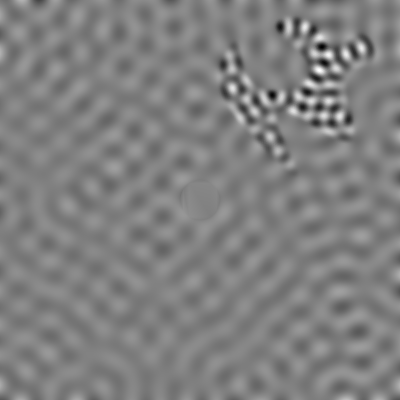
\includegraphics[height=3cm,width=0.95\textwidth]{test_irregular_2_real.png}
			\caption{Wavefield image}
		\end{subfigure}\quad
		\begin{subfigure}[h]{0.25\textwidth}
			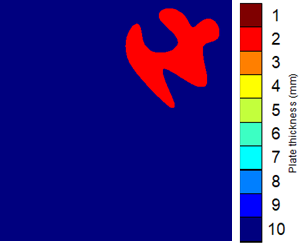
\includegraphics[height=3cm,width=\textwidth]{test_irregular_2_truth.png}
			\caption{Ground truth}
		\end{subfigure}
		\begin{subfigure}[h]{0.25\textwidth}
			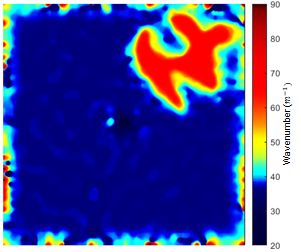
\includegraphics[height=3cm,width=\textwidth]{test_irregular_2_aws.png}
			\caption{AWS prediction}
		\end{subfigure}
		\begin{subfigure}[h]{0.25\textwidth}
			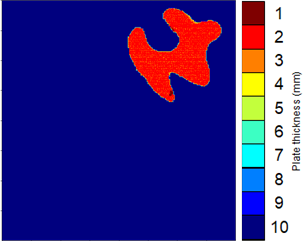
\includegraphics[height=3cm,width=\textwidth]{test_irregular_2_cnn.png}
			\caption{CNN prediction}
		\end{subfigure}
		\caption{AWS v. CNN results for an irregular shape}
		\label{fig:aws comparison}
	\end{figure}
	\tableofcontents
	\newpage
	\section{Project overview}
	The project overview map shown in figure \ref{fig:overview} provides an ordered high-level view of the many tasks performed in this project.
	\begin{figure}[H]
		\centering
		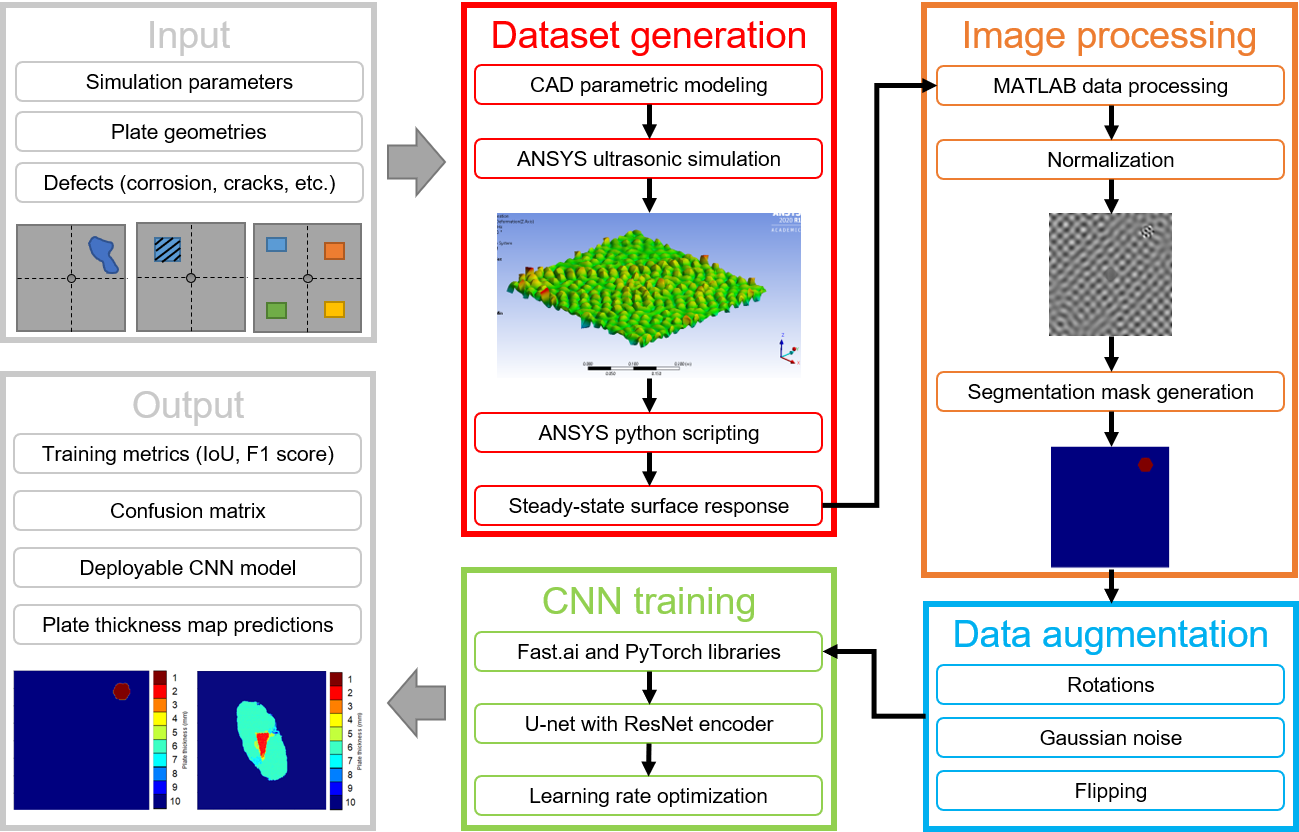
\includegraphics[width=\textwidth]{project_overview.png}
		\caption{Project overview map}
		\label{fig:overview}
	\end{figure}
	The next section will walk through each of these steps in greater detail. In general,
	\begin{enumerate}
		\item \textbf{Input:} A simulation scheme was brainstormed by hand that tried to incorporate as many scenarios in the dataset as possible. The final trained CNN model is only as good as the data it is given, so this is perhaps the most important step for improving the CNN model's accuracy and robustness. Among the parameters that must be chosen are excitation frequency, plate dimensions, size and shape of defects, quantity and quality of defects, location and thickness of defects, transducer location, and mesh size and other simulation parameters.
		
		\item \textbf{Dataset generation:} Once a simulation scheme was developed on paper, the parameters must be input into CAD modeling to generate hundreds of CAD \textit{.step} geometry files. SpaceClaim was used within ANSYS workbench to generate these models in a \textit{for} loop by iteratively adjusting different dimensions. Most other CAD software packages can perform similar parametric modeling. Once the models were generated, a Python script was used to run hundreds of ANSYS harmonic response simulations on the geometry \textit{.step} files. The real and imaginary parts of the plate's surface deformation response (representing the steady-state simple sinusoidal oscillations at every mesh node point) were exported to \textit{.txt} files by ANSYS ADPL commands.
		
		\item \textbf{Image processing:} The real and imaginary parts of the steady-state deformation response of the plate were then read directly into a MATLAB script for further processing. MATLAB was used to filter out surface mesh points, interpolate to an evenly-spaced grid, normalize the data, and generate a grayscale wavefield image for all of the real, imaginary, and magnitude steady-state response of the plate. MATLAB also was used to automatically generate segmentation masks of the plate indicating the location and thickness of defects on a pixel by pixel basis.
		
		\item \textbf{Data augmentation:} The \textit{numpy} and \textit{scikit-learn} Python libraries were used to rotate and add Gaussian noise to all of the wavefield images to increase the dataset size.
		
		\item \textbf{CNN training:} The \textit{Fast.ai} and \textit{PyTorch} machine learning Python libraries were used to build and train a U-net CNN architecture for an image segmentation task. The popular \textit{ResNet} architecture was pre-trained on the ImageNet database and loaded as an encoder into our U-net model. The \textit{Fast.ai} recommended protocols for training a CNN model were followed where applicable. \textit{Fast.ai} follows the \textit{fit one cycle} mantra, where the CNN model with pretrained weights and biases is frozen and the last few fully-connected layers are trained on the new dataset (our wavefield dataset) using an optimal learning rate. The CNN model is then mostly unfrozen and trained again on our dataset to refine the internal layers.
		
		\item \textbf{Output:} The trained CNN model reports its final intersection-over-union (IoU) value and F1 score (dice coefficient). These training accuracy metrics can be used to benchmark performance against other published CNN models. The trained CNN model can be exported to a pickle (\textit{.pkl}) file to be deployed on new systems for running inference on new images. The output of running inference on a new image is a color-coded segmentation mask that indicates the predicted local plate thickness on a pixel by pixel level.
	\end{enumerate}
	
	\section{Detailed project workflow}
	This section will seek to provide a more comprehensive set of procedures that can be followed to replicate this project from scratch. It will also point out common pitfalls we experienced along the way, as well as existing problems that still need to be addressed.
		\subsection{Software and installation details}
		All software used in this project is detailed in table \ref{table:software} below, as well as installation and documentation links. All dataset generation and image processing were performed on a Windows 10 system; data augmentation and CNN training were performed on a Debian-based Linux virtual machine.
		\begin{table}[H]
		\centering
		\captionsetup{margin=1cm}
		\caption{Software and hardware details and installation links}
		\renewcommand{\arraystretch}{1.5}
		\begin{tabular}{| c | c | c |}
		\hline
	 	\textbf{Name} & \textbf{Version} & \textbf{Link} \\ \hline \hline
	 	Python & 3.7.6 & \url{https://docs.anaconda.com/anaconda/install/}\\ \hline
		Fast.ai & 1.0.61 & \url{https://github.com/fastai/fastai1} \\ \hline
		PyTorch & 1.4.0 & (installed with Fast.ai)\\ \hline
		numpy & 1.18.1 & (installed with Fast.ai)\\ \hline
		matplotlib & 3.2.1 & (installed with Fast.ai)\\ \hline
		PIL & 7.1.2 &(installed with Fast.ai) \\ \hline
		Jupyter notebook & - & (installed with Fast.ai)\\ \hline
		skimage & 0.17.2 & \url{https://scikit-image.org/docs/dev/install.html}\\ \hline
		NVIDIA driver & 418.87 & NVIDIA Tesla P100-PCIE-16GB GPU\\ \hline
		CUDA & 10.1 & \url{https://developer.nvidia.com/cuda-zone} \\ \hline
		MATLAB & R2019a & Statistics, Parallel computing toolbox, Engine API for Python \\ \hline
		ANSYS & 19.1 & \url{https://www.ansys.com/academic}\\ \hline
		Dropbox & 10.3.0 & \url{https://www.dropbox.com/developers/documentation} \\ \hline
		\end{tabular}\\
		\label{table:software}
		\end{table}
		ANSYS and MATLAB licenses are required (proprietary software). The Statistics toolbox for MATLAB is required for segmentation mask generation. The Parallel Computing toolbox is recommended for processing speed-up, but not required. The MATLAB Engine for Python was used to further automate the workflow between ANSYS simulations and MATLAB post-processing, but this is not required. ANSYS scripting uses the IronPython 2.7 version of the generic Python language. The Anaconda distribution of Python may be used for all deep learning software tools, (not required; you can use a generic Python installation). The Dropbox API can be used with a free or paid subscription. The NVIDIA GPU and CUDA toolkit were used on a cloud computing virtual machine through Google Cloud Platform (GCP). GCP is a paid service with a free trial period; you may use this or any other suitable hardware acceleration platform for deep learning (Google Collab, Kaggle, personal computer, etc.). More details on setting up a GCP deep learning instance with Fast.ai are included in the \textit{project\_workflow.pptx} slides in the documentation folder. The Fast.ai Python library and all dependencies (PyTorch, numpy, PIL, etc.) may be installed with the conda or pip package managers (see the Fast.ai installation link). It is recommended that these are installed on your CUDA-enabled machine within a Python virtual environment (whether through Anaconda or another virtual environment tool, like virtualenv).
		
		\subsection{Directory structure}
		Most of the source code files used in the project are heavily dependent on the underlying directory structure. Not only will this directory structure keep your project organized, but it will allow source code files to access the data they need to run. Everything is coded relative to the project's root folder, which can be placed anywhere in the user's home filesystem. The following list outlines the project's directory structure and its usage.
		\begin{itemize}
			\item[] \textbf{/DeepWaves} \hfill \textit{DeepWaves project root folder}
			\begin{itemize}
				\item[] \textbf{/ansys} \hfill \textit{ANSYS project folder}
				\begin{itemize}
					\item[] \textbf{/DeepWaves\_files} \hfill \textit{ANSYS generated file storage for .wbpj}
					\begin{itemize}
						\item[] \textbf{/dp0/SYS/MECH} \hfill \textit{Location of ADPL output data.txt files}
						\begin{enumerate}
							\item[] real.txt \hfill \textit{Real part of steady-state deformation response}
							\item[] imaginary.txt \hfill \textit{Imaginary part of steady-state deformation response}
						\end{enumerate}
					\end{itemize}
					\item[] DeepWaves.wbpj \hfill \textit{ANSYS workbench project file; run Python script here}
				\end{itemize}
				\item[] \textbf{/data} \hfill \textit{MATLAB reads all data.txt files from this folder}
				\begin{itemize}
					\item[] example\_sim\_real.txt \hfill \textit{Location where real.txt is moved and renamed}
					\item[] example\_sim\_imaginary.txt \hfill \textit{Location where imaginary.txt is moved and renamed}
					\item[] another\_sim\_real.txt
					\item[] another\_sim\_imaginary.txt
				\end{itemize}
				\item[] \textbf{/documentation} \hfill \textit{All doc files like this one}
				\item[] \textbf{/geometry} \hfill \textit{ANSYS reads all .step geometry files from here}
				\begin{itemize}
					\item[] example\_sim.step
					\item[] another\_sim.step
				\end{itemize}
				\item[] \textbf{/images} \hfill \textit{MATLAB outputs wavefield images here and}
				\begin{itemize}
					\item[] example\_sim\_real.png \hfill \textit{CNN reads image dataset from here}
					\item[] example\_sim\_imaginary.png
					\item[] example\_sim\_magnitude.png
					\item[] another\_sim\_real.png 
					\item[] another\_sim\_imaginary.png
					\item[] another\_sim\_magnitude.png
				\end{itemize}
				\item[] \textbf{/labels} \hfill \textit{MATLAB outputs segmentation masks here and}
				\begin{itemize}
					\item[] example\_sim\_mask.png \hfill \textit{CNN reads segmentation masks from here}
					\item[] another\_sim\_mask.png
				\end{itemize}
				\item[] \textbf{/logs} \hfill \textit{Store all log files during script execution}
				\begin{itemize}
					\item[] run\_sims.log \hfill \textit{ANSYS simulation log file}
				\end{itemize}
				\item[] \textbf{/mat} \hfill \textit{Store all complex deformation matrices as .mat files here}
				\begin{itemize}
					\item[] example\_sim\_vqz.mat
					\item[] another\_sim\_vqz.mat
				\end{itemize}
				\item[] \textbf{/models} \hfill \textit{CNN exports model .pth and .pkl files here}
				\begin{itemize}
					\item[] training\_run.pth \hfill \textit{.pth files rely on access to dataset to reload CNN model}
					\item[] training\_run.pkl \hfill \textit{.pkl files are deployable trained CNN models}
				\end{itemize}
				\item[] \textbf{/src} \hfill \textit{All Python and MATLAB source code files here}
				\begin{itemize}
					\item[] \textbf{/CAD\_scripts} \hfill \textit{Directory containing ACT CAD modeling code snippets}
					\item[] ACT\_mech\_script.py \hfill \textit{Runs harmonic response sim in ANSYS ACT console}
					\item[] augment.py \hfill \textit{Creates new augmented images from dataset}
					\item[] codes.txt \hfill \textit{Read by CNN and MATLAB to enumerate plate thickness classes}
					\item[] display\_dir.m \hfill \textit{MATLAB function to display images in a folder}
					\item[] filter\_defect.m \hfill \textit{Uses kmeans clustering to find plate defects in ANSYS node data}
					\item[] noise.py \hfill \textit{Script to add Gaussian noise to images}
					\item[] norm\_batch.m \hfill \textit{Batch normalization over entire dataset}
					\item[] plot\_wavefield.m \hfill \textit{Generates wavefield images and segmentation masks}
					\item[] process\_images.m \hfill \textit{Calls plot\_wavefield.m over entire dataset}
					\item[] run\_matlab.py \hfill \textit{Uses MATLAB Python engine to call .m files}
					\item[] run\_sims.py \hfill \textit{Automates ANSYS simulation process}
					\item[] unet\_train\_JE.ipynb \hfill \textit{Jupyter notebooks to train CNN : JE method}
					\item[] unet\_train\_0\_004\_KH.ipynb \hfill \textit{KH method}
					\item[] unet\_train\_0\_0009\_KH.ipynb \hfill \textit{KH method}
				\end{itemize}
				\item[] \textbf{/test} \hfill \textit{CNN runs inference on all test images in here}
				\begin{itemize}
					\item[] test\_image\_real.png
					\item[] another\_test.png
				\end{itemize}
			\end{itemize}
		\end{itemize}
		It is noted that not all features are tested across different systems. Different installations and versions may cause different problems in running the code. All code used in running ANSYS simulations especially might need to be tweaked depending on your system. It is also unsure how well ANSYS project files translate between systems (all details for setup are provided below though). Data exported from ANSYS is heavy in memory requirements. If a large number of simulations are meant to be run overnight, one might consider setting up a cloud storage account with Dropbox and utilizing the Dropbox API to automatically move simulation files off of the host computer to prevent filling up or crashing the hard drive, (run\_matlab.py has some inspiration for this task if desired). The \textit{directory\_structure.txt} and \textit{source\_files.txt} files in the documentation folder provide more detail on this section.
		\subsection{Input}
		Table \ref{table:input} shows all of the parameters accounted for in this study. Several parameters, like plate geometry and material, were kept constant throughout the study. A total of 8 \textquote{rounds} of datasets were generated by deciding how and which parameters changed in each round.
		\begin{table}[H]
		\centering
		\captionsetup{margin=1cm}
		\caption{Geometry and simulation parameters for dataset generation}
		\renewcommand{\arraystretch}{1.5}
		\begin{tabular}{| c | c |}
		\hline
	 	\textbf{Parameter} & \textbf{Value} \\ \hline \hline
	 	Mesh size & $2\ \si{\milli\metre}$ \\ \hline
		Plate size & $400\times 400\ \si{\milli\metre}$ \\ \hline
		Plate Material & Aluminum alloy (ANSYS generic) \\ \hline
		Plate thickness & $1-10\ \si{\milli\metre}$ \\ \hline
		Transducer frequency & $80\ \si{\kilo\hertz}$ \\ \hline
		Transducer location & Variable \\ \hline
		Number of defects & $1-4$ \\ \hline
		Plate thickness at defect & $1-9\ \si{\milli\metre}$ \\ \hline
		Defect location & Variable \\ \hline
		Defect shape & Variable \\ \hline
		Defect size & Variable \\ \hline
		\end{tabular}\\
		\label{table:input}
		\end{table}
		The \textit{simulation\_tracker.xlsx} spreadsheet and the \textit{simulation\_plan.pptx} slides provide more detail on the 8 rounds of simulations performed in this study. Future studies should account for a greater variety of the dataset parameters listed above, including plate material, size, and transducer frequency. It is also noted here that there are several unaccounted parameters not listed here that could be studied in the future, including the shape, size, and number of transducers.
		\subsection{Dataset generation}
		Once a simulation scheme is developed by hand from the previous \textquote{Input} section, there are 3 main steps in generating the physical data from the devised simulation scheme: modeling the geometry in computer-aided design (CAD) software, setting up a finite element analysis (FEA) solver, and automating the FEA solver.
			\subsubsection{CAD parametric modeling}
			Most CAD software packages (Solidworks, Inventor, SpaceClaim, etc.) have a way for users to set certain geometry dimensions (length, depth, etc.) as variable parameters that are programmatically varied to generate multiple geometry models in an incremental fashion. This form of parametric modeling was performed in SpaceClaim in this study to quickly generate all of the geometry models devised in the simulation scheme (usually on the order of 100-200 unique geometries per round). If the reader is using a different CAD package, they might seek the appropriate resources to perform similar modeling in their respective CAD package. \bigskip
			
			In the SpaceClaim modeler provided within ANSYS workbench, ANSYS offers the \textit{ANSYS Customization Toolkit} (ACT) console for interactive Python programming within the CAD software. The \textit{src/CAD\_scripts} directory contains several ACT Python code snippets that were run directly within the ACT console to generate all of the geometry \textit{.step} files used in this study. The reader may use these code snippets as references in writing their own parametric modeling scripts within SpaceClaim to generate their unique geometry files for their simulation schemes. It is noted here that documentation online for the ACT Python API is very limited; the best way to quickly write working Python code within the ACT console is to use the journaling feature provided within ANSYS to record all interaction with the CAD graphical user interface (GUI) and generate Python code to replicate all recorded GUI interactions (mouse clicks, opening menus, selecting faces, etc.). \bigskip
			
			For the sake of simplicity and compliance with the ANSYS simulation described in the next sections, each geometry should be modeled as a plate-like structure on the XY plane with its center at the 3D origin of the CAD software design space, and the depth of the plate extruded outward in the positive z-direction. There should be a small cylindrical extrusion of $1\ \si{\milli\metre}$ in the positive z-direction off of the plate's top face. This small cylinder is meant to model the physical ultrasonic transducer on the plate (it was given a diameter of $40\ \si{\milli\metre}$ in this study). The simulations assume the top face of the transducer is located at the greatest z-coordinate value in the geometry (always true if you follow the setup described here). Figure \ref{fig:geometry} shows a screenshot of a typical plate geometry modeled in this fashion.
			\begin{figure}[H]
			\centering
			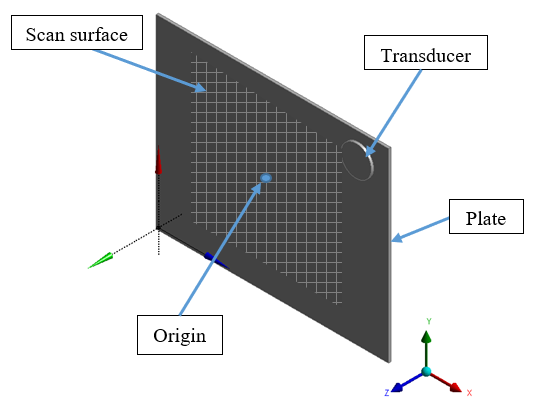
\includegraphics[width=0.8\textwidth]{plate_geometry.png}
			\caption{Example plate geometry with transducer on plate's surface}
			\label{fig:geometry}
			\end{figure}
			After completing this task, the reader should have geometry \textit{.step} files for each desired model setup created during the simulation scheme. These geometry files should be located in the \textit{geometry} folder.
			\subsubsection{Setting up the ANSYS FEA solver}
			Now that all plate geometry files are created, the steady-state ultrasonic excitation response of the plate can be obtained by a harmonic response simulation in ANSYS Mechanical. The procedure for setting up this simulation follows previous work by O'Dowd et al.\ \cite{o2016exploring} The simulation setup procedures are included in the \textit{ansys\_sim\_tutorial.docx} file in the documentation folder. Any of the \textit{.step} files generated in the previous section can be loaded in for the geometry instead of recreating the geometry as indicated in the simulation procedures. The ANSYS generic Aluminum Alloy material was used for this study. The procedures include the ADPL commands that must be inserted into ANSYS Mechanical to export the steady-state response data of the plate. Once the ANSYS setup procedures are completed, save the workbench project in the \textit{ansys} directory under the project root folder.
			\subsubsection{Automating ANSYS simulations}
			Once the simulation has been setup in ANSYS and saved, it is now ready to load the geometry \textit{.step} files, run the harmonic response simulation, and export the steady-state response data files. Depending on the platform and system, these tasks take several minutes to complete per geometry file. For this study, this workflow was automated to sequentially load geometry files into the ANSYS workbench project, run the harmonic response simulation, export the data, and optionally run the data through Matlab image processing and offload to Dropbox cloud storage; the \textit{run\_sims.py} script performs these tasks programmatically. The reader must make a few edits to this script file before running:
			\begin{enumerate}
			\item Change the SetUserPathRoot() DirectoryPath argument to the absolute path to your project root folder on your system (i.e. C:\textbackslash Users\textbackslash eckelsjd\textbackslash DeepWaves).
			\item (Optional) Install Matlab engine for Python and uncomment the two Python os system calls in the main \textit{for} loop which execute the \textit{run\_matlab.py} Python script.
			\item (Optional) Install the Matlab statistics toolbox and edit the \textit{cmd} variable from the previous step to specify what kind of segmentation mask you would like to automatically generate. See the Matlab \textit{plot\_wavefield.m} source code file for options. This is the Matlab function called from within Python via the arguments specified in the \textit{cmd} variable. Also reference the \textit{exec\_matlab()} function in the \textit{run\_matlab.py} source code file for more information.
			\item (Optional) Install the Dropbox Python API, setup a Dropbox account, and copy the Python API account key into the \textit{run\_matlab.py} script. Follow online tutorials and the inline comments in the script to adjust the \textit{upload} function so that it properly uploads files to your Dropbox account. Uncomment the calls to the \textit{upload} function in main() to move your files off the hard drive to your Dropbox account. Note: you should feel comfortable reading through the \textit{run\_matlab.py} source code and making edits so that the Dropbox API can properly find your account and move all associated files.
			\item Open ANSYS workbench. Go to File$\rightarrow$scripting$\rightarrow$Run Script file and select \textit{run\_sims.py}. The script will begin loading all \textit{.step} files from the geometry folder and running the simulation in ANSYS mechanical. You will see data .txt files show up in the data folder as simulations complete. 
			\item If you opted to run Matlab image processing and/or Dropbox file offloading, you will see a command window pop up and indicate its progress, and image files (and segmentation masks, if indicated) will begin populating the images and labels folders, respectively. All errors that occur while scripting will be written to the \textit{run\_sims.log} file in the logs folder, and you may also see errors appear in the ANSYS workbench GUI. Errors that occur during Matlab image processing or Dropbox file handling are harder to catch; these errors will cause the command window to close abruptly and ANSYS workbench to stop executing. If this happens, you will need to test the \textit{run\_matlab.py} file separately from ANSYS workbench, perhaps in a Windows command prompt running interactive Python. Errors with Matlab are likely due to incorrect arguments passed to \textit{plot\_wavefield.m}. Errors with Dropbox are likely due to incorrect file handling or account authentication errors (incorrect keys, IDs, namespaces, etc.). 
			\end{enumerate}
		\subsection{Image processing}
		The default output of the ANSYS automation performed in the previous section is a \textit{real.txt} and an \textit{imaginary.txt} file for each simulation performed, representing the real and imaginary deformation response data, respectively. These data files will be located in the data folder, and will be renamed based on the filename of the \textit{.step} files. For example, \textit{geometry1.step} will produce two data files in the data folder: \textit{geometry1\_real.txt} and \textit{geometry1\_imaginary.txt}. These filenames can be passed directly to the Matlab \textit{plot\_wavefield.m} function, along with a few other parameters, to generate the wavefield images for the data (real, imaginary, and magnitude), and optionally create a segmentation mask image. This function can also optionally export a complex-valued deformation matrix .mat file by uncommenting the appropriate lines in the source code. These complex matrices are used in AWS processing to generate AWS wavenumber map predictions. All generated image files are saved to the images folder; all segmentation masks are saved to the labels folder; all .mat files are saved to the mat folder. See the source code of \textit{plot\_wavefield.m} for more details. \bigskip
		
		There are three ways to perform the Matlab image processing:
		\begin{enumerate}
		\item Call \textit{plot\_wavefield.m} on one set of data directly. This is mostly useful for debugging and checking output of a single simulation.
		\item Run the \textit{process\_images.m} Matlab script. This simply calls \textit{plot\_wavefield.m} in a \textit{for} loop; make changes to the \textit{plot\_wavefield.m} function call within \textit{process\_images.m} to change the arguments. The script will generate wavefield images for all data files in the data folder automatically; this requires all complementary real.txt and imaginary.txt files to be present in the data folder at the time of execution. This script allows you the option to perform batch normalization over the entire dataset before generating the wavefield images as well. In order to use the \textit{parfor} loop in the script, you must have the Matlab Parallel Computing toolbox; if you don't, just change the \textit{parfor} loop to a normal \textit{for} loop (with slower run times).
		\item Make the optional changes listed in the previous section to automatically generate wavefield images from within the ANSYS Python script directly.
		\end{enumerate}
		The wavefield images generated during image processing are used as the raw input to the convolutional neural network (CNN) for training. In this study, only the real surface response wavefield images were used for CNN training. A segmentation mask \textquote{label} was generated for each real wavefield by specifying the \textquote{default} argument to the \textit{plot\_wavefield.m} function. The ground truth segmentation mask was generated by specifying the \textquote{color} argument instead (only for visualization and comparison). The default segmentation label images (in the labels folder) appear completely black. Each pixel is given a numeric value equivalent to its class identifier. In this study, there were 10 plate thickness classes to identify in each image on a pixel by pixel basis, as summarized in table \ref{table:classes}.
		\begin{table}[H]
		\centering
		\captionsetup{margin=1cm}
		\caption{10 thickness classes with numeric class identifiers}
		\renewcommand{\arraystretch}{1.5}
		\begin{tabular}{| c | c |}
		\hline
	 	\textbf{Thickness class} & \textbf{Class identifier (pixel value)} \\ \hline \hline
	 	$10\ \si{\milli\metre}$ & 0 \\ \hline
	 	$9\ \si{\milli\metre}$ & 1 \\ \hline
	 	$8\ \si{\milli\metre}$ & 2 \\ \hline
	 	$7\ \si{\milli\metre}$ & 3 \\ \hline
	 	$6\ \si{\milli\metre}$ & 4 \\ \hline
	 	$5\ \si{\milli\metre}$ & 5 \\ \hline
	 	$4\ \si{\milli\metre}$ & 6 \\ \hline
	 	$3\ \si{\milli\metre}$ & 7 \\ \hline
	 	$2\ \si{\milli\metre}$ & 8 \\ \hline
	 	$1\ \si{\milli\metre}$ & 9 \\ \hline
		\end{tabular}\\
		\label{table:classes}
		\end{table}
		In a given $10\ \si{\milli\metre}$ thick plate with no defects, every single pixel value in the segmentation label image would have an RGB value of $(0,0,0)$, equivalent to its class identifier. If a corrosive defect was introduced to the back of the plate, causing the thickness of the plate in that region to be reduced to $7\ \si{\milli\metre}$, then all pixel values in that region of the segmentation label image would have an RGB value of $(3,3,3)$. Thus, the CNN will be given wavefield images of a plate and it will be told (via the label images) which wave patterns and regions in the image correspond to what plate thickness value. In this way, the CNN will be trained to classify local plate thickness based on local wave patterns and features, irrespective of the wave modes present.
			\subsubsection*{Segmentation mask limitations}
			There are several limiting cases that cause problems with the current automatic segmentation mask generation. The segmentation mask section of the \textit{plot\_wavefield.m} file has several comments on how the code works. In general, 3D mesh node point coordinates (X,Y,Z) are grouped according to their Z-value. Nodes on the surface of the plate have a Z-value equal to the plate thickness. The filename of the data specifies the thickness of the plate at the surface, as well as at the defect location. From the filename alone, if you have a 10mm thick plate with a defect of thickness 4mm, the code will parse this information out. At the defect location, there will be a flat surface at a Z-value equal to the plate thickness minus the thickness at the defect (a Z-value of 6mm in this case). Using the \textit{kmeans} function in the Matlab Statistics toolbox, the node points at this Z-value are grouped into a cluster, and all node points at this Z-value that are far away from the cluster are filtered out. Now we have obtained the location and depth of the defect from the filename alone. However, the mesh node (X,Y,Z) coordinates are not in line with the uniform grid of the wavefield image; we must map these random mesh points to the uniform grid. This mapping is done using the Matlab built-in function \textit{dsearchn}. This function takes all of the mesh node coordinates and maps them to the closest points on the uniform grid. However, the mapping is rather sparse because the uniform grid is much more refined than the mesh node points. After a series of blurring, edge detection, and image hole-filling, the uniform grid is a segmentation mask that is white at the defect and black everywhere else. We can create a segmentation mask like this for every thickness class, set the white spots equal to the appropriate class identifier, and logically AND each thickness segmentation mask together to combine into one segmentation label image for the CNN. This same process is done for the ground truth images, just with 3 channels for RGB visualization. \bigskip
			
			Here are the current limitations of this approach:
			\begin{enumerate}
			\item Must have the Matlab Statistics toolbox.
			\item Increased processing time.
			\item Filename must follow conventions for the segmentation masks to generate properly. For each new round, you must give some indication of the plate thickness and the number and thickness of defects. Future work would eliminate these dependencies somehow.
			\item The \textit{kmeans} function filters only 1 cluster by default. This method only supports segmenting when there is exactly one defect at a given thickness, not for example when there are two 1mm defects in different locations on the plate. To fix this, you would need some way for Matlab to automatically detect how many clusters there are, or to include how many clusters there are in the filename so you can pass a cluster argument to \textit{kmeans}.
			\item Performance is only reliably good when there is only one defect total present in the plate at any thickness. When there is more than one defect, the mesh node points often cluster in locations other than the surface of the defect, which throws off the \textit{kmeans} algorithm for filtering out only the defect's mesh node points. There are cases where there might be a 1mm defect and a 5mm defect somewhere else in the same plate, and the segmentation mask is still generated just fine. This just needs more testing and debugging to figure out the real problem behind this limitation. One possible solution is to only export ANSYS mesh node point data at select regions or Z-values rather than having Matlab do all of the filtering.
			\item Along with the previous limitation, overlapping defects often overwrite each other and produce incorrect segmentation masks. The order in which the logical ANDs are performed to combine different thickness masks affects the performance on this problem.
			\end{enumerate}
			If the reader comes across a case where the segmentation mask is not generating properly, then it most likely falls in one of the categories above. The reader should always visually check the generated masks to make sure the code is performing correctly. If there is no way to correctly generate the mask using this code, then Matlab can be used to hardcode the location and depth of the defects and draw colored shapes on a uniform grid. However, this method would be rather difficult with irregular shapes. It's best to stick to regular shapes, like circles and squares, if you would prefer to make segmentation masks this way. It is also possible, albeit rather tedious, to use Matlab's image processing tool, or some other labeling software to generate segmentation masks by hand. Despite the automatic mask generation's limitations, it is still much more adaptable to changing geometry. Future work would improve upon the limitations listed above.
		\subsection{Data augmentation}
		After generating all wavefield images and segmentation labels, the overall dataset size should be increased by augmentation. Several common data augmentation techniques, such as blurring, warping, lighting, and tilting would cause physical wave pattern features to change in the wavefield images in an undesirable way. In this study, four data augmentation techniques were identified to avoid these warping effects: adding Gaussian noise, rotating 180 degrees, vertical flipping, and horizontal flipping. All plate geometries were designed to only have defects in the upper right quadrant of the plate. A 180 degree rotation was applied to every image to double the dataset size. Then, Gaussian noise was added to every image in the new dataset to double in size again. An original dataset size of 200 images would increase to 800 images, while still only having to perform 200 simulations. During CNN training, horizontal and vertical flipping were applied randomly to the dataset between training epochs. In this way, the CNN was exposed to defects in all four quadrants of the plate. The \textit{augment.py} Python script uses the \textit{numpy} and \textit{scikit-learn} Python libraries to perform the data augmentation described here. All new augmented images were saved in the images folder with new filenames. Rotations were also applied to segmentation labels and saved back into the labels folder.
		\subsection{CNN training}
		The completed raw dataset consisted of all original real wavefield images and augmentations in the images folder along with all corresponding segmentation label images in the labels folder. The dataset was uploaded to a Google Cloud Platform (GCP) virtual machine (VM) with GPU-acceleration capability. One of the source code Jupyter notebooks were opened on the VM and accessed by static IP addressing from the host machine. All Fast.ai CNN training procedures were followed cell by cell in the Jupyter notebook, including loading the dataset and labels, splitting the dataset 20/80 into validation and training sets, loading a U-net CNN architecture with a pre-trained ResNet encoder, searching and selecting an optimal learning rate, and training the CNN on the dataset for several epochs. The CNN must be able to find corresponding label images based on the filenames of the wavefield dataset images. For enhanced training, the CNN was saved to \textit{.pth} files and loaded later after changing several training parameters. \bigskip
		
		See the \textit{training\_instructions} files in the documentation directory for more details on performing the CNN training. The two training instructions documents correspond to two different methods performed in this study for CNN training. The procedures described in this document and in \textit{training\_instructions\_JE.txt} are to be used with the \textit{unet\_train\_JE.ipynb} Jupyter notebook. The \textit{training\_instructions\_KH.docx} file outlines procedures to use the \textit{unet\_train\_KH.ipynb} Jupyter notebooks. The \textit{source\_files.txt} document also provides more detail on using all source files mentioned in this section.
		\subsection{Output}
		After training, the CNN was exported to a \textit{.pkl} file for deployment on another system. The CNN model displayed its intersection-over-union (IoU) value and F1 score (dice coefficient) during training to indicate its accuracy on the validation set. The model's performance on the validation set was also quantified by a confusion matrix on each class value. Test images were generated similar to the original dataset and were passed to the trained CNN for inference prediction. The CNN outputted a thickness prediction map in a linear-thickness color scale, indicating the regions of the plate with different thickness values. An example of this output is shown in figure \ref{fig:aws comparison}.
	\section{Future work}
	After reaching the end of the previous section, you have made it as far as we did at the time of writing. This section will speculate on things we wish we had time for, or places we believe the project could go in the future.
		\subsection{Addressing current limitations}
		Several limitations have been discussed throughout this document with respect to software bugs and hardware limitations. Areas of special interest that need more work are generating segmentation masks automatically from ANSYS data, thinning the data exported from ANSYS to decrease storage requirements, and searching for alternatives to ANSYS simulations to speed up simulation processing time (or just throw more GPUs at it).
		\subsection{Comprehensive dataset}
		In this study, a total of 8 different rounds of simulations were performed to account for as many physical scenarios as possible. This effort was extensive, but certainly not exhaustive. There are several real-world experimental test cases that fall outside of the parameters our simulations accounted for. To improve the robustness of the CNN model, the training dataset must be larger and more comprehensive. Some cases to consider include changing plate dimensions, variable transducer frequencies, multiple transducers on the same plate, non-plate-like structures, training on experimental data in addition to simulated data, structures where higher wave modes (other than A0 and S0) are present, thicker plates, unbounded plates, plates with multiple defects in multiple orientations and dimensions, etc.
		\subsection{Regression}
		The task at hand is an image segmentation problem, which is inherently a classification problem, just classification on the pixel level. The authors of the current study started here as a proof-of-concept. Ultimately, however, the problem at hand of identifying defects in a plate is a regression problem, where defects are allowed to take on any value in a continuous range, not just one of a set few discrete values. It is not currently known if there are existing CNN models out in the field that perform regression on an image segmentation task. Perhaps further computer science research into the data being passed to the fully-connected layers at the end of the image segmentation CNN could indicate a way to output classifications on a continuous scale rather than a discrete one. This would be an excellent area of further research, and is most recommended by the authors.
		\subsection{CNN model refinement}
		None of the authors have great experience in the field of machine learning and neural networks. The Fast.ai library was chosen as a machine learning platform because of its short on-ramp in generating decent results with little prior training. However, Fast.ai hides most of the inner-workings of the network (intentionally) from the user. Further optimizations of the network would require more training and a shift away from Fast.ai into a more mature platform like TensorFlow or PyTorch, where customization is more open and achievable. Once this shift is made, more state-of-the-art models, like the recent Refine-net image segmentation model \cite{8618363}, can be implemented in code and trained on our dataset for improved performance.
		\subsection{CNN training refinement}
		In conjunction with the previous statement on CNN model refinement, moving to a more mature platform would also allow further testing and refinement on training hyperparameters, such as weight decay, batch size, and learning rate to improve model accuracy. Most of these hyperparameters were left default in this study, but future work should experiment with these values and find the optimal parameters for training the CNN model.
		
	\newpage
	\bibliographystyle{ieeetran}
    \bibliography{References}
\end{document}